\documentclass[../main.tex]{subfiles}

\pagestyle{main}
\renewcommand{\chaptermark}[1]{\markboth{\chaptername\ \thechapter\ (#1)}{}}
\renewcommand{\thechapter}{\Roman{chapter}}
\setcounter{chapter}{1}

\begin{document}




\chapter{Symmetry and Group Theory in Chemistry}
\setcounter{section}{2}
\section{Module 3: Symmetry Elements and Operations}
\begin{itemize}
    \item \marginnote{1/13:}He will upload lecture slides in advance in the future.
    \item An object is symmetric if one part is the same as other parts.
    \item The symmetry of discrete objects is described using \textbf{Point Symmetry}.
    \item \textbf{Point groups} ($\sim 32$ for molecules) provide us with a way to indicate the symmetry unambiguously.
    \item Point groups have symmetry about a single point at the center of mass of the system.
    \item Extended objects (e.g., crystals) have \textbf{translational symmetry} described by \textbf{Space groups}\footnote{Not covered in this course.} (230 total).
    \item Reading: \textcite{bib:MiesslerFischerTarr} Chapter 4 and \url{https://en.wikipedia.org/wiki/Molecular_symmetry}.
    \item \textbf{Symmetry elements}: Geometric entities about which a \textbf{symmetry operation} can be performed. In a point group, all symmetry elements must pass through the center of mass (the point).
    \item \textbf{Symmetry operation}: The action that produces an object identical to the initial object.
\end{itemize}
\begin{tchart}{1.2}{Element}{Operation}
    Identity, $E$ & nothing\\
    Rotation axis, $C_n$ & $n$-fold rotation\\
    Improper rotation axis, $S_n$ & $n$-fold improper rotation\\
    Plane of symmetry, $\sigma$ & Reflection\\
    Center of symmetry, $i$ & Inversion\\
\end{tchart}
\begin{itemize}
    \item \textbf{Identity}: Does nothing to the object, but is necessary for mathematical completeness.
    \item \textbf{$\bm{n}$-fold rotation}: A rotation of $\ang{360}/n$ about the $C_n$ axis ($n\in[1,\infty)$).
    \begin{itemize}
        \item In \ce{H2O}, there is a $C_2$ axis, so we can perform a $2$-fold ($\ang{180}$) rotation to get the same molecule.
        \begin{itemize}
            \item Remember, because of quantum mechanical properties, the hydrogens are indistinguishable so when we rotate it $\ang{180}$, we cannot tell it apart from the unrotated molecule.
        \end{itemize}
        \item Rotations are considered positive in the counter-clockwise direction.
        \item Each possible rotation operation is assigned using a superscript integer $m$ of the form ${C_n}^m$. $m$ is the number of sequential applications.
        \item The rotation ${C_n}^n=E$ is equivalent to the identity operation (nothing is moved).
        \item Linear molecules have an infinite number of rotational options $C_\infty$ because any rotation on the molecular axis will give the same arrangement.
    \end{itemize}
    \item \textbf{Principal axis}: The highest order rotation axis.
    \begin{itemize}
        \item By convention, the principal axis is assigned to the $z$-axis if we are using Cartesian coordinates.
    \end{itemize}
    \item \textbf{Reflection}: Exchanges one half of the object with the reflection of the other half.
    \item \textbf{Vertical mirror plane}: A mirror plane that contains the principal axis. \emph{Also known as} $\bm{\sigma_v}$.
    \item \textbf{Horizontal mirror plane}: A mirror plane that is perpendicular to the principal axis. \emph{Also known as} $\bm{\sigma_h}$.
    \item \textbf{Dihedral mirror planes}: A special type of $\sigma_v$ that is between sides or planes. \emph{Also known as} $\bm{\sigma_d}$.
    \begin{itemize}
        \item For example, we might have vertical mirror planes in the $xz$- or $yz$-planes. In this case, the dihedral planes would contain the lines $y=\pm x$.
    \end{itemize}
    \item Two successive reflections are equivalent to the identity operation.
    \item \textbf{Inversion}: Every part of the object is reflected through the inversion center, which must be at the center of mass of the object.
    \begin{itemize}
        \item $(x,y,z)\xrightarrow{i}(-x,-y,-z)$.
    \end{itemize}
    \item \textbf{$\bm{n}$-fold improper rotation}: This operation involves a rotation of $\ang{360}/n$ followed by a reflection perpendicular to the axis. It is a single operation and is labeled in the same manner as "proper" rotations. \emph{Also known as} $\bm{{S_n}^m}$.
    \begin{figure}[h!]
        \centering
        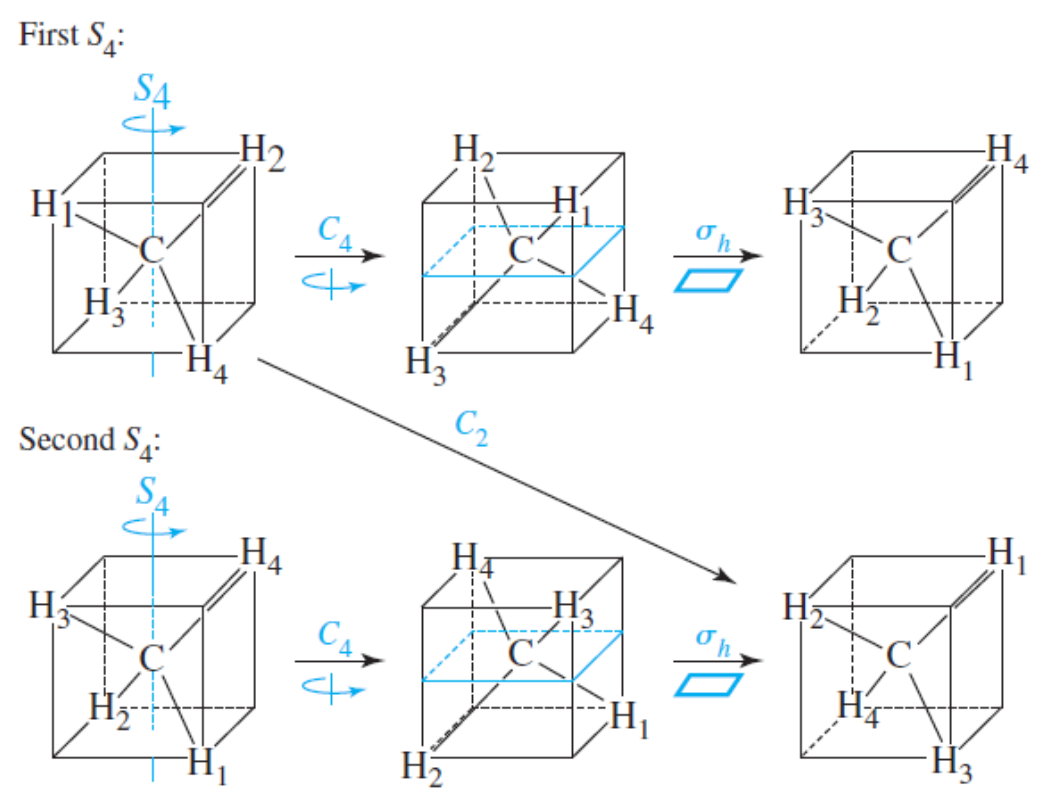
\includegraphics[width=0.4\linewidth]{ExtFiles/methaneImproperRotation.png}
        \caption{Methane's $S_4$ symmetry.}
        \label{fig:methaneImproperRotation}
    \end{figure}
    \begin{itemize}
        \item Methane has $S_4$ symmetry.
        \item Note that $S_1=\sigma_h$, $S_2=i$, and sometimes $S_{2n}=C_n$. In methane, for example, ${S_4}^2=C_2$.
        \item Applied to a triangular prism, is a good example.
        \item If $n$ is even, we have $n$ unique operations. There should be $C_{n/2}$.
        \item If $n$ is odd, we have $2n$ unique operations. There should be $C_n$ and $\sigma_h$.
    \end{itemize}
    \item The absence of an $S_n$ axis is the defining symmetry property of \textbf{chiral} molecules.
    \begin{itemize}
        \item Formerly, we learned that chiral molecules should not have mirror planes and inversion centers.
        \item Rigorously, chiral molecules must not have any improper rotation axes.
    \end{itemize}
\end{itemize}



\section{Module 4: Symmetry Point Groups}
\begin{itemize}
    \item Identifying the point groups:
    \begin{enumerate}
        \item Determine if the symmetry is special (e.g., octahedral).
        \item Determine if there is a principal rotation axis.
        \item Determine if there are rotation axes perpendicular to the principal axis.
        \item Determine if there are mirror planes.
        \item Assign point groups.
    \end{enumerate}
    \item High symmetry and low symmetry groups are the most difficult to identify.
    \item High symmetry:
    \begin{itemize}
        \item Perfect tetrahedral ($T_d$), e.g., \ce{P4} and \ce{CH4}.
        \item Perfect octahedral ($O_h$), e.g., \ce{SF6}.
        \item Perfect icosahedral ($I_h$), e.g., \ce{C60}.
    \end{itemize}
    \item Low symmetry:
    \begin{figure}[h!]
        \centering
        \begin{subfigure}[b]{0.24\linewidth}
            \centering
            \footnotesize
            \chemfig[cram width=3pt,cram dash width=0.5pt,cram dash sep=1.3pt,atom sep=7mm]{*8(<(<[:-120]F_3)=>(>:[:-30]F_2)=<(<[:60]F_1)=>(>:[:150]F_4)=)}
            \caption{$S_4$.}
            \label{fig:lowSymmetrya}
        \end{subfigure}
        \begin{subfigure}[b]{0.24\linewidth}
            \centering
            \footnotesize
            \chemfig{Cl-[1]C(<[:120]H)(>:[:60]F)-[7]Cl}
            \caption{$C_s$}
            \label{fig:lowSymmetryb}
        \end{subfigure}
        \begin{subfigure}[b]{0.24\linewidth}
            \centering
            \footnotesize
            \chemfig{H-[1]C(>:[3]Br)(<[:170]Cl)-C(<[7]Br)(>:[:-10]Cl)-[1]H}
            \caption{$C_i$}
            \label{fig:lowSymmetryc}
        \end{subfigure}
        \begin{subfigure}[b]{0.24\linewidth}
            \centering
            \footnotesize
            \chemfig{C(-[:-30]Br)(<[:-110]Cl)(>:[:-150]F)-[2]H}
            \caption{$C_1$}
            \label{fig:lowSymmetryd}
        \end{subfigure}
        \caption{Low symmetry point groups.}
        \label{fig:lowSymmetry}
    \end{figure}
    \begin{itemize}
        \item Only an improper axis: $S_n$.
        \item Only a mirror plane: $C_s$.
        \item Only an inversion center: $C_i$.
        \item No symmetry: $C_1$.
    \end{itemize}
    \item $C_n$ groups:
    \begin{itemize}
        \item Only a $C_n$ axis. Note that conformation is important.
    \end{itemize}
    \item $C_{nh}$ groups have a $C_n$ axis and a $\sigma_h$ reflection plane (such as \ce{B(OH)3}).
    \begin{itemize}
        \item \ce{H2O2} has $C_{2h}$ symmetry.
    \end{itemize}
    \item All symmetry elements are listed in the top row of the corresponding characters table (Appendix C in \textcite{bib:MiesslerFischerTarr}).
    \item $C_{nv}$ groups have a $C_n$ axis and a $\sigma_v$ reflection plane.
    \begin{itemize}
        \item \ce{NH3} has $C_{3v}$ symmetry.
        \item \ce{CO} has $C_{\infty v}$ symmetry since there are an infinite number of both $C_n$ axes and $\sigma_v$ mirror planes.
    \end{itemize}
    \item $D_{nh}$ groups: A $C_n$ axis, $n$ perpendicular $C_2$ axes, and a $\sigma_h$ reflection plane.
    \begin{itemize}
        \item \ce{BH3} has $D_{3h}$ symmetry.
        \item A square prism has $D_{4h}$ symmetry.
        \item \ce{CO2} has $D_{\infty h}$ symmetry.
    \end{itemize}
    \item $D_n$ groups: A $C_n$ axis, $n$ perpendicular $C_2$ axes, and no mirror planes.
    \begin{itemize}
        \item A 3-bladed propeller has $D_3$ symmetry.
    \end{itemize}
    \item $D_{nd}$ groups: A $C_n$ axis, $n$ perpendicular $C_2$ axes, and a $\sigma_d$.
    \begin{itemize}
        \item Ethane in the staggered conformation has $D_{3d}$ symmetry.
    \end{itemize}
    \item Local symmetry:
    \begin{itemize}
        \item Sometimes, rigorous math analysis needs to be adjusted to physical reality.
        \item If a cyclopentane ring is bonded through the center to \ce{Mn(CO)3}, this molecule has only $C_s$ symmetry.
        \item However, spectroscopically, there is fast rotation about the \ce{Mn-Cp} bond. This means that the \ce{Mn(CO)3} fragment exhibits pseudo-$C_{3v}$ symmetry while the \ce{C5H5} ligand exhibits pseudo-$C_{5v}$ symmetry.
        \item Often, the absolute symmetry of a molecule is very low, but the interactions are far away from the centers of interest, and do not perturb them significantly.
        \item If we have platinum as a central atom bonded to two chlorines and two \ce{P(Et)3} groups, this molecule technically has $C_1$ symmetry due to the orientations of atoms within \ce{R} groups (staggered), but IR spectroscopy is characteristic of highly symmetric species ($D_{2h}$).
    \end{itemize}
\end{itemize}




\end{document}